%%%%%%%%%%%%%%%%%%%%%%%%%%%%%%%%%%%%%%%%%%%%%%%%%%%%%%%%%%%%%%%%%%%%%%
% Lớp 10 | Đại số tổ hợp | Hoán vị. Chỉnh hợp. Tổ hợp
% Dạng 0D8?2-6: Bài toán có yếu tố hình học
% Số câu: 34  (sinh tự động bởi tach_cau.py; từ nay thầy sửa trực tiếp file này)
%%%%%%%%%%%%%%%%%%%%%%%%%%%%%%%%%%%%%%%%%%%%%%%%%%%%%%%%%%%%%%%%%%%%%%

%%%%%%%%%%%%%%%% TRẮC NGHIỆM 4 PHƯƠNG ÁN %%%%%%%%%%%%%%%%

% nguồn: MaHoaNH_TracNghiem_Lop10
\begin{ex}%[0D8N2-6]%[ma:11e0c124]
	Số giao điểm tối đa của  $10$ đường thẳng phân biệt là
	\choice 
		{$50$} 
		 {$100$}
		 {$120$}
		{\True $45$} 
	 \loigiai{
		Số giao điểm  tối đa của $10$ đường thẳng phân biệt là $\mathrm{C}_{10}^2=45$.
	} 
\end{ex}

% nguồn: MaHoaNH_TracNghiem_Lop10
\begin{ex}%[0D8N2-6]%[ma:9ce00d02]
	Trong mặt phẳng cho tập hợp gồm $25$ điểm phân biệt. Có bao nhiêu véc-tơ khác véc-tơ $\overrightarrow{0}$ có điểm đầu và điểm cuối thuộc  tập hợp điểm này?
	\choice 
		 {$50$}
		 {$300$}
		{\True $600$} 
		{$625$} 
	 \loigiai{
		Số véc-tơ khác $\overrightarrow{0}$ có điểm đầu và điểm cuối được tạo ra bởi $25$ điểm phân  biệt là $\mathrm{A}_{25}^2=600$ véc-tơ.
	 }
\end{ex}

% nguồn: MaHoaNH_TracNghiem_Lop10
\begin{ex}%[0D8N2-6]%[ma:b745b1a7]
	Cho $10$ điểm phân biệt cùng nằm trên một đường tròn, số tam  giác tạo thành là
	 \choice
		{$720$} 
		{\True  $120$}
		{$82$} 
		{$186$} 
	\loigiai{ 
		Vì  các điểm đã cho phân biệt và nằm trên một đường tròn nên không có $3$ điểm nào thẳng hàng.\\
		Số tam giác được tạo thành là số cách chọn ra $3$ trong  số $10$ điểm đã cho.\\
	Do đó, số tam giác tạo  thành bằng $\mathrm{C}_{10}^3=120$.}
\end{ex}

% nguồn: MaHoaNH_TracNghiem_Lop10
\begin{ex}%[0D8N2-6]%[ma:7a68cc78]
	Trong mặt phẳng cho $12$ điểm  phân biệt trong đó không có $3$ điểm nào thẳng hàng. Số tam giác có $3$ đỉnh là $3$ trong $12$ điểm đã cho là
	 \choice
		{$12^3$} 
		 {\True $\mathrm{C}_{12}^3$}
		 {$12!$}
		 {$\mathrm{A}_{12}^3$}
	 \loigiai{
	Mỗi tam giác tạo thành là một tổ  hợp chập $3$ của $12$ phần tử.\\
	Vậy số tam giác  có $3$ đỉnh là $3$ trong $12$ điểm đã cho là $\mathrm{C}_{12}^3$.
	} 
\end{ex}

% nguồn: MaHoaNH_TracNghiem_Lop10
\begin{ex}%[0D8N2-6]%[ma:b4a1849d]
	Trên mặt phẳng cho lục giác $ABCDEF$. Hỏi có  bao nhiêu véc-tơ khác véc-tơ $\overrightarrow 0 $ và có điểm đầu, điểm cuối là 2 trong 6 đỉnh của lục giác đã cho?
	\choice 
		{$36$} 
		 {\True $30$}
		{$11$} 
		{$25$} 
	 \loigiai{
	Mỗi véc-tơ tạo thành là một chỉnh hợp chập $2$ của $6$ phần tử.\\ 
	Vậy số véc-tơ thoả mãn bài toán là $\mathrm{A}_6^2=  30$.
	} 
\end{ex}

% nguồn: MaHoaNH_TracNghiem_Lop10
\begin{ex}%[0D8H2-6]%[ma:1756a5ac]
	Trong  mặt phẳng cho tập hợp $S$ gồm $10$ điểm phân biệt, trong đó không có $3$ điểm nào thẳng hàng. Có bao nhiêu tam giác có $3$ đỉnh đều thuộc $S$?
	 \choice
		{\True  $120$}
		 {$720$}
		 {$3628800$}
		{$59049$} 
	\loigiai{Số tam giác  có $3$ đỉnh được lập từ $S$ là $\mathrm{C}_{10}^{3}=120$.}
\end{ex}

% nguồn: MaHoaNH_TracNghiem_Lop10
\begin{ex}%[0D8H2-6]%[ma:8e56d707]
	Số giao điểm tối đa của $5$ đường  tròn phân biệt là
	 \choice
		{$20$} 
		 {$22$}
		 {$18$}
		 {\True $10$}
	\loigiai{ 
	Cứ hai đường tròn phân biệt sẽ có tối đa $2$ giao điểm. Do đó số giao điểm tối đa của $5$ đường  tròn phân biệt là $\mathrm{C}_5^2=10$.}
\end{ex}

% nguồn: MaHoaNH_TracNghiem_Lop10
\begin{ex}%[0D8H2-6]%[ma:72e109eb]
	Cho $2$ đường thẳng $a$ và $b$ song song với nhau. Trên đường thẳng $a$ ta chọn $10$ điểm phân biệt và trên đường thẳng  $b$ ta chọn $11$ điểm phân biệt. Có bao nhiêu hình thang được tạo thành từ các điểm đã chọn ở trên?
	 \choice
		 {\True $2475$}
		{$2512$} 
		 {$304$}
		{$406$} 
	 \loigiai{
		Chọn $2$ điểm phân biệt trên $a$ và $2$ điểm phân biệt  trên $b$.\\
	Ta  có $\mathrm{C}_{10}^2\cdot\mathrm{C}_{11}^2=2475$ hình thang được tạo thành từ các điểm đã cho.}
\end{ex}

% nguồn: MaHoaNH_TracNghiem_Lop10
\begin{ex}%[0D8H2-6]%[ma:6045eca0]
	Cho đa giác đều gồm $n$ đỉnh $(n \geq 3,n\in \mathbb{N})$. Số tam giác có $3$  đỉnh là $3$ đỉnh của đa giác đã cho là
	 \choice
		{$\mathrm{A}^3_n$} 
		{\True  $\mathrm{C}^3_n$}
		{$\dfrac{\mathrm{C}^3_n}{3!}$} 
		{$n!$} 
	\loigiai{ 
		Số tam giác có $3$  đỉnh là $3$ đỉnh của đa giác đã cho là $\mathrm{C}^3_n$.
	} 
\end{ex}

% nguồn: MaHoaNH_TracNghiem_Lop10
\begin{ex}%[0D8H2-6]%[ma:68ae002a]
	Trong  mặt phẳng cho một tập hợp gồm $6$ điểm phân biệt. Có bao nhiêu vectơ khác vectơ $\overrightarrow 0$ có điểm đầu và điểm cuối thuộc tập hợp điểm này?
	\choice 
		 {$15$}
		{$12$} 
		 {$1\,440$}
		 {\True $30$}
	\loigiai{ 
		Mỗi cặp sắp thứ tự gồm hai điểm $\left(A, B\right)$ cho ta một vectơ có điểm đầu $A$ và điểm cuối $B$ và ngược lại. Như vậy, mỗi vectơ có thể xem là một chỉnh hợp chập $2$ của tập hợp  $6$ điểm đã cho.\\
		Suy ra có $\mathrm{A}_6^2=30$  cách.
	} 
\end{ex}

% nguồn: MaHoaNH_TracNghiem_Lop10
\begin{ex}%[0D8H2-6]%[ma:7aa6211a]
	Cho một đa giác đều $20$ đỉnh nội tiếp $1$ đường tròn. Chọn ngẫu nhiên $4$ đỉnh của đa  giác. Hỏi có bao nhiêu cách chọn để đa giác tạo thành là một hình chữ nhật?
	\choice 
		 {$60$}
		{$38$} 
		{\True  $45$}
		 {$30$}
	\loigiai{ 
		Để tạo thành một hình chữ nhật cần có $2$ đường chéo đi qua tâm đường tròn nội tiếp đa giác đều. Đa giác có $20$ cạnh  sẽ có $10$ đường chéo qua tâm.\\
		Vậy  số hình chữ nhật tạo thành là $\mathrm{C}_{10}^2=45$.
	 }
\end{ex}

% nguồn: MaHoaNH_TracNghiem_Lop10
\begin{ex}%[0D8H2-6]%[ma:bce5672c]
	Cho $n$ điểm phân biệt. Xét tất cả các véc-tơ  khác $\overrightarrow{0}$, có điểm đầu và điểm cuối là các điểm đã cho. Số véc-tơ thoả mãn là
	 \choice
		 {$n$}
		{$n-1$} 
		{$\dfrac{n(n-1)}{2}$} 
		 {\True $n(n-1)$}
	\loigiai{ 
		Mỗi véc-tơ khác $\overrightarrow{0}$  là một chỉnh hợp chập $2$ của $n$ điểm đã cho.\\
		Vậy số véc-tơ thoả  mãn bài toán là $\mathrm{A}_n^2=n(n-1)$.
	} 
\end{ex}

% nguồn: MaHoaNH_TracNghiem_Lop10
\begin{ex}%[0D8H2-6]%[ma:3e6151ed]
	Số đường chéo của một  lục giác lồi là.
	\choice 
		{$6$} 
		 {$18$}
		{\True  $9$}
		 {$30$}
	\loigiai{ 
		Số đoạn thẳng tạo bởi hai điểm bất kỳ từ các đỉnh của hình  lục giác lồi là $\mathrm{C}_6^2=15$.\\
		Trong số các đoạn thẳng này có $6$ đoạn thẳng là cạnh và $15-6=9$ đoạn  thẳng là đường chéo.
	} 
\end{ex}

% nguồn: MaHoaNH_TracNghiem_Lop10
\begin{ex}%[0D8H2-6]%[ma:19dec333]
	Có thể tạo thành bao nhiêu vectơ khác vectơ không từ mười điểm phân biệt trên mặt phẳng? 
	\choice 
		{$10!$} 
		{$\mathrm{C}_{10}^2$} 
		 {$10$}
		 {\True $\mathrm{A}_{10}^2$}
	\loigiai{ 
		 Mỗi vectơ khác vectơ không được tạo thành bằng cách lấy hai điểm từ mười điểm đã cho và phân biệt thứ tự điểm đầu và điểm cuối. \\
		Như vậy, mỗi vectơ  là một chỉnh hợp chập $2$ của $10$. \\
		Vậy số các  vectơ tạo thành là $\mathrm{A}_{10}^2$.
	 }
\end{ex}

% nguồn: MaHoaNH_TracNghiem_Lop10
\begin{ex}%[0D8H2-6]%[ma:8857fdda]
	Nếu một đa giác lồi có $44$ đường chéo  thì đa giác đó có bao nhiêu cạnh?
	\choice 
		{$8$} 
		 {$10$}
		 {$9$}
		{\True  $11$}
	\loigiai{ 
		Gọi $n$  là số đỉnh của đa giác $(n\ge 3)$. \\
		Tổng số đường chéo và số cạnh của đa giác trên là $\dfrac{\mathrm{A}_n^2}{2}$, trong đó $n$ là số cạnh của  đa giác. \\
		Ta  có
		\begin{align*}
			&\dfrac{\mathrm{A}_n^2}{2}=n+44\\ 
			 \Leftrightarrow &\dfrac{n!}{2!(n-2)!}=n+44\\
			\Leftrightarrow  &\dfrac{1}{2}n(n-1)-n-44=0\\
			\Leftrightarrow  &n^2-3n-88=0\\
			 \Leftrightarrow &\hoac{ & n=11 \text{ (nhận)}\\
			& n=-8\text{  (loại)}. }
		\end{align*}
		Vậy đa giác đó có  $11$ cạnh.
	} 
\end{ex}

% nguồn: MaHoaNH_TracNghiem_Lop10
\begin{ex}%[0D8V2-6]%[ma:2271d8a2]
	Một đa giác đều có số đường chéo  gấp đôi số cạnh. Hỏi đa giác đó có bao nhiêu cạnh?
	\choice 
		{\True  $7$}
		 {$6$}
		 {$8$}
		 {$5$}
	 \loigiai{
		Giả  sử đa giác lồi có $n$ cạnh $\left(n\in \mathbb{N}, n\ge 3\right)$.\\
		Khi đó số đường chéo của đa giác là  $\mathrm{C}_n^2-n=\dfrac{n(n-1)}{2}-n=\dfrac{n(n-3)}{2}$.\\
		Theo đề bài  ta có $\dfrac{n(n-3)}{2}=2n\Leftrightarrow n^2-7n=0\Leftrightarrow \hoac{&n=0 &&(\text{loại}) \\&n=7 &&(\text{nhận}).}$\\
	Vậy đa giác có $7$ cạnh thì số đường chéo gấp đôi số cạnh.} 
\end{ex}

% nguồn: MaHoaNH_TracNghiem_Lop10
\begin{ex}%[0D8V2-6]%[ma:f44767a4]
	Cho đa giác đều có $15$ đỉnh, gọi $M$ là tập tất cả các tam giác có ba đỉnh là ba đỉnh của đa giác đã cho. Trong số các tam giác đó có bao nhiêu tam giác là tam giác cân  nhưng không phải là tam giác đều?
	\choice 
		 {$64$}
		{$70$} 
		 {$72$}
		 {\True $90$}
	 \loigiai{
		Gọi  $O$ là tâm đường tròn ngoại tiếp đa giác đều.\\
		Xét một đỉnh $A$ bất kì của đa giác đều: có 7 cặp đỉnh của đa giác đối xứng với nhau qua $OA$, hay có $7$ tam  giác cân tại đỉnh $A$.\\
		Như vậy, với mỗi đỉnh  của đa giác có $7$ tam giác nhận nó làm đỉnh tam giác cân.\\
		 Số tam giác đều có ba đỉnh là ba đỉnh của đa giác là $\dfrac{15}{3}=5$ tam giác.\\
		Tuy nhiên, trong các tam giác cân đã xác định ở trên có cả tam giác đều, do mọi tam giác đều thì đều cân tại ba đỉnh nên các tam giác đều  được đếm ba lần.\\
		Suy ra số tam giác cân nhưng không phải tam giác đều có ba đỉnh là ba đỉnh của đa  giác đã cho là $7\cdot 15-3\cdot 5=90$.
	 }
\end{ex}

% nguồn: MaHoaNH_TracNghiem_Lop10
\begin{ex}%[0D8V2-6]%[ma:06cf59f7]
	Cho tập $A$ gồm $n$ điểm phân biệt trên mặt phẳng sao cho không có $3$ điểm nào thẳng  hàng. Tìm $n$ sao cho số tam giác có $3$ đỉnh lấy từ $3$ điểm thuộc $A$ gấp đôi số đoạn thẳng được nối từ $2$ điểm thuộc $A$.
	\choice 
		{$n=6$} 
		 {$n=12$}
		{\True $n=8$} 
		{$n=15$} 
	\loigiai{Điều  kiện $n\in\mathbb{N}$, $n\geq 3$.\\
		Số tam  giác có $3$ đỉnh thuộc tập $A$ là $\mathrm{C}_n^3$.\\
		Số đoạn thẳng được nối từ $2$ điểm thuộc tập $A$ là $\mathrm{C}_n^3$.\\ 
		Theo đề bài ta có \begin{eqnarray*}
		 &&\mathrm{C}_n^3=2\mathrm{C}_n^2\\
		&\Leftrightarrow&  \dfrac{n(n-1)(n-2)}{6}=2\cdot\dfrac{n(n-1)}{2}\\
		 &\Leftrightarrow& n-2=6\Leftrightarrow n=8.
	\end{eqnarray*}
Vậy $n=8$.} 
\end{ex}

% nguồn: MaHoaNH_TracNghiem_Lop10
\begin{ex}%[0D8V2-6]%[ma:7c6cefa4]
	Cho hai đường thẳng $d_1$ và $d_2$ song song với nhau. Trên $d_1$ có $10$ điểm phân biệt, trên  $d_2$ có $7$ điểm phân biệt. Hỏi có bao nhiêu tam giác mà ba đỉnh của nó được chọn từ $17$ điểm vừa nói trên.
	 \choice
		 {\True $525$}
		{$680$} 
		 {$155$}
		{$600$} 
	 \loigiai{
		Trường hợp 1: Tam giác có một đỉnh thuộc  $d_1$ và hai đỉnh thuộc $d_2$.\\
		Số cách  chọn một điểm trong $10$ thuộc $d_1$ là $\mathrm{C}_{10}^1$.\\
		Số cách chọn bộ hai điểm trong $7$ điểm  thuộc $d_2$ là $\mathrm{C}_7^2$.\\
		TH này  có $\mathrm{C}_{10}^1\cdot \mathrm{C}_7^2$ tam giác.\\
		Trường hợp 2: Tam giác có một đỉnh thuộc  $d_2$ và hai đỉnh thuộc $d_1$.\\
		Số cách chọn  bộ hai điểm trong $10$ thuộc $d_1$ là $\mathrm{C}_{10}^2$.\\
		Số cách chọn một điểm trong $7$ điểm thuộc  $d_2$ là $\mathrm{C}_7^1$.\\
		 TH này có $\mathrm{C}_{10}^2\cdot \mathrm{C}_7^1$ tam giác.\\
		Vậy  có tất cả $\mathrm{C}_{10}^1\cdot \mathrm{C}_7^2+\mathrm{C}_{10}^2\cdot \mathrm{C}_7^1=525$ tam giác thỏa mãn yêu cầu bài toán.
	} 
\end{ex}

% nguồn: MaHoaNH_TracNghiem_Lop10
\begin{ex}%[0D8V2-6]%[ma:69bf8b4a]
	Cho hai đường thẳng $d_1$ và $d_2$  song song với nhau. Trên $d_1$ có $10$ điểm phân biệt, trên $d_2$ có $n$ điểm phân biệt ($n\geq 2$). Biết rằng có $1725$ tam giác có các đỉnh là ba trong số các điểm thuộc $d_1$ và $d_2$ nói trên. Tìm tổng các chữ số của $n$.
	 \choice
		{$3$} 
		{\True $6$} 
		{$4$} 
		 {$5$}
	 \loigiai{
		Ta thấy cứ một điểm bất kì trên đường thẳng $d_1$  với hai điểm phân biệt trên $d_2$ hoặc cứ một điểm bất kì trên đường thẳng $d_2$ với hai điểm phân biệt trên $d_1$ tạo thành một tam giác.\\
		Do đó số tam giác có $3$ đỉnh trong số các điểm thuộc  $d_1$ và $d_2$ là $10\cdot\mathrm{C}_n^2+n\mathrm{C}_{10}^2$.
		Ta có \begin{eqnarray*}
		 10\cdot\mathrm{C}_n^2+n\mathrm{C}_{10}^2=1725 &
		\Leftrightarrow  & 10\cdot\dfrac{n(n-1)}{2}+45n=1725\\
		&\Leftrightarrow & 5n\left(n-1\right)+45n-1725=0\\ 
		&\Leftrightarrow & 5n^2+40n-1725=0\\ 
		&\Leftrightarrow &\hoac{&n=15  \\&n=-23.}
	\end{eqnarray*}
Vậy $n=15$ và $1+5=6$.} 
\end{ex}

% nguồn: MaHoaNH_TracNghiem_Lop10
\begin{ex}%[0D8V2-6]%[ma:44a54c02]
	Bé Minh có một bảng hình chữ nhật gồm $6$ hình vuông đơn vị, cố định không xoay như hình vẽ. Bé muốn dùng $3$ màu để tô tất cả các cạnh của các hình vuông đơn vị, mỗi cạnh tô một lần sao cho mỗi hình vuông đơn vị được tô bởi đúng $2$ màu, trong đó mỗi màu tô đúng $2$ cạnh. Hỏi bé Minh có tất cả bao nhiêu cách tô màu  bảng?
	 \choice
		 {$4\,374$}
		{$139\,968$} 
		 {$756$}
		{\True $15\,552$} 
	 \loigiai{
		Tô màu theo  nguyên tắc.\\
		Tô $1$ ô vuông $4$ cạnh: chọn $2$ trong $3$ màu, ứng với $2$ màu được  chọn có $6$ cách tô.\\
		 (Bổ sung: chọn $2$ ô trong $4$ ô, tô $1$ màu, còn $2$ ô còn lại tô màu thứ $2$ nên có $\mathrm{C}_4^2=6$ cách).\\
		Do đó, có $6\cdot  3=18$ cách tô.\\
		(Ô vuông này phải chọn ô ở giữa thì mới tạo ra $3$ ô vuông ở bước $2$ có  một cạnh đã được tô).\\
		Tô $3$ ô vuông có $3$ cạnh chưa được tô (một cạnh đã được tô trước đó): ứng với $1$ ô vuông này, do một cạnh đã được tô màu nên có $3$ cách tô màu này cho $1$ trong $3$  cạnh còn lại theo màu của cạnh đã tô trước đó.\\
		Chọn $1$ trong $2$ màu còn lại tô $2$ cạnh còn lại, có $3\cdot  2=6$ cách tô.\\
		Do đó có $6^3$ cách  tô.\\
		Tô $2$ ô vuông còn  lại có $2$ cạnh đã được tô màu trước đó (có $2$ cạnh đã được tô trước đó) bỏ: ứng với $1$ ô vuông có $2$ cách tô màu $2$ cạnh ($2$ cạnh tô trước cùng màu hay khác nhau không ảnh hưởng số cách tô).\\
		 Do đó có $2^2$ cách tô.\\
		Vậy có  $18\cdot 6^3\cdot 4=15\,552$ cách tô.
	 }
\end{ex}

% nguồn: MaHoaNH_TracNghiem_Lop10
\begin{ex}%[0D8V2-6]%[ma:175fcec2]
	Cho đa giác đều có $100$ đỉnh. Hỏi có  bao nhiêu tam giác tù được tạo thành từ các đỉnh của đa giác đều đã cho?
	 \choice
		{$58\,800$} 
		{$1\,176$} 
		{$235\,200$} 
		 {\True $117\,600$}
	 \loigiai{
	\immini  {
		 Đánh số các đỉnh là $\mathrm{A}_1$, $\mathrm{A}_2$, {\dots}, $\mathrm{A}_{100}$.\\
		Xét đường kính $\mathrm{A}_1 \mathrm{A}_{51}$ của đường tròn ngoại tiếp đa giác đều đã cho. Đường kính này chia $98$ đỉnh còn lại của đa giác đều làm hai phần, mỗi phần $49$ đỉnh: từ  $\mathrm{A}_2$ đến $\mathrm{A}_{50}$ và từ $\mathrm{A}_{52}$ đến $\mathrm{A}_{100}$.\\
		Khi đó mỗi tam giác có dạng $\mathrm{A}_1 \mathrm{A}_i \mathrm{A}_j$ là tam giác tù (tại $\mathrm{A}_i$ hoặc  $\mathrm{A}_j$) khi và chỉ khi $\mathrm{A}_i$, $\mathrm{A}_j$ cùng nằm trên nửa đường tròn tức là cùng thuộc một phần mô tả ở trên.
		 }{
		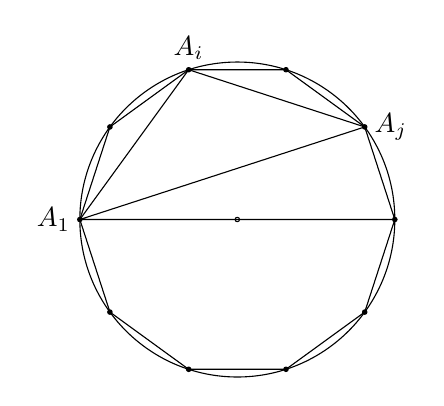
\begin{tikzpicture}[scale =0.8,line join=round,line cap=round,>=stealth]
				\def\r{2.5} \def\gy{120} 
				\draw (0,0) circle (1pt)  circle (\r);
				\foreach \i  in {0,36,...,324}
				\filldraw  (\i:\r) circle (1pt)-- (\i+36:\r);
				\draw (180:\r) node[left]{$A_1$}--(108:\r)  node[above]{$A_i$}--(36:\r) node[right]{$A_j$}--cycle
					(180:\r)--(0:\r); 
			\end{tikzpicture}
		} 
		 \noindent Chọn đỉnh $\mathrm{A}_1$ có $100$ cách.\\
		Chọn  nửa đường tròn có $2$ cách.\\
		 Chọn $2$ đỉnh $\mathrm{A}_i$, $\mathrm{A}_j$ có $\dfrac{\mathrm{A}_{49}^2}{2!}$ cách.\\
		Giả  sử tam giác $\mathrm{A}_1 \mathrm{A}_i \mathrm{A}_j$ là tam giác tù tại $\mathrm{A}_i$ thế thì tam giác $\mathrm{A}_j \mathrm{A}_i \mathrm{A}_1$ cũng được đếm thêm $1$ lần vào số các tam giác tù kể trên. Tuy nhiêu hai tam giác này chỉ là một, vậy ta đã đếm lặp hai lần.\\
		Tóm lại số tam giác tù có thể lập được là  $\dfrac{100\cdot 2\cdot \dfrac{\mathrm{A}_{49}^2}{2!}}{2}=117\,600$.
	} 
\end{ex}


%%%%%%%%%%%%%%%% ĐÚNG/SAI %%%%%%%%%%%%%%%%

% nguồn: MaHoaNH_DungSai_Lop10
\begin{ex}%[0D8N2-6]%[ma:42cbd57e]
	Cho lục giác $ABCDEF$. Chọn khẳng định đúng trong các khẳng  định sau.
	\choiceTF 
		{\True Số véc-tơ khác $\overrightarrow{0}$ có điểm đầu, điểm cuối là hai  trong $6$ đỉnh của lục giác là $30$}
		{Số véc-tơ khác  $\overrightarrow{0}$ có điểm đầu, điểm cuối là hai trong $6$ đỉnh của lục giác là $15$}
		{\True Số tam  giác tạo thành từ $6$ đỉnh của lục giác là $20$}
		{Số tam giác tạo thành từ $6$ đỉnh của  lục giác là $120$}
	 \loigiai{
		\begin{itemize}
			\item Số véc-tơ khác $\overrightarrow{0}$ có điểm đầu, điểm cuối là hai trong $6$ đỉnh của  lục giác là $\mathrm{A}_6^2=30$.
			\item Số tam giác tạo thành từ  $6$ đỉnh của lục giác là $\mathrm{C}_6^3=20$.
		\end{itemize}
	} 
\end{ex}

% nguồn: MaHoaNH_DungSai_Lop10
\begin{ex}%[0D8N2-6]%[ma:80a9daa7]
	Cho $8$ điểm trong đó không có $3$ điểm nào thẳng hàng. Chọn khẳng định đúng trong các khẳng  định sau.
	 \choiceTF
		{\True Số tứ giác tạo thành từ $8$ đỉnh trên  là $70$}
		{\True Số  tam giác tạo thành từ $8$ đỉnh trên là $56$}
		{Số đoạn thẳng tạo thành từ $8$ đỉnh trên là  $56$}
		{\True Số đoạn thẳng tạo thành từ $8$ đỉnh trên là  $28$}
	\loigiai{ 
		\begin{itemize}
			\item Số tứ giác tạo thành từ $8$ đỉnh trên là $\mathrm{C}_8^4=70$. 
			\item Số tam  giác tạo thành từ $8$ đỉnh trên là $\mathrm{C}_8^3=56$.
			\item Số đoạn thẳng tạo thành từ $8$ đỉnh trên là  $\mathrm{C}_8^3=28$.
		\end{itemize}
	 }
\end{ex}

% nguồn: MaHoaNH_DungSai_Lop10
\begin{ex}%[0D8V2-6]%[ma:0d5fc78e]
	Cho đa  giác đều $12$ đỉnh.
	 \choiceTF
		{Số đoạn thẳng có hai đầu mút được tạo nên từ $12$  đỉnh trên là $\mathrm{A}_{12}^{2}$}
		{\True Số vectơ khác vectơ $\overrightarrow{0}$ được tạo nên từ $12$  đỉnh trên là $\mathrm{A}_{12}^{2}$}
		{Số đường  chéo của đa giác là $52$}
		{Số hình chữ  nhật có $4$ đỉnh được lập từ $12$ đỉnh trên là $\mathrm{C}_{12}^{4}$}
	 \loigiai{
		\begin{itemchoice}
			\itemch Một đoạn thẳng  được tao nên từ $2$ điểm và $2$ điểm này không có thứ tự nên số đoạn thẳng được tạo nên từ $12$ đỉnh trên là $\mathrm{C}_{12}^{2}=66$.
			\itemch Một vectơ khác vectơ $\overrightarrow{0}$ được tạo nên từ $2$ điểm và  $2$ điểm này có thứ tự nên số vectơ khác vectơ $\overrightarrow{0}$ được tạo nên từ $12$ đỉnh trên là $\mathrm{A}_{12}^{2}=132$.
			\itemch Cứ $2$ đỉnh của đa giác sẽ tạo thành một đoạn thẳng  (bao gồm cả cạnh và đường chéo).\\
			Khi đó số đoạn thẳng là  $\mathrm{C}_{12}^{2}=66$.\\
			Số đường chéo là  $66-12=54$.
			\itemch Đa giác đều $12$ đỉnh thì có số đường chéo  đi qua tâm là $\dfrac{12}{2}=6$.\\
			Mỗi hình chữ nhật được tạo nên từ hai  đường chéo đi qua tâm nên số hình chữ nhật là $\mathrm{C}_{6}^{2}=15$.
		\end{itemchoice}
	} 
\end{ex}


%%%%%%%%%%%%%%%% TRẢ LỜI NGẮN %%%%%%%%%%%%%%%%

% nguồn: MaHoaNH_TraLoiNgan_Lop10
\begin{bt}%[0D8H2-6]%[ma:09cc8326]
	Cho một đa giác đều $n$ đỉnh ($n\in \mathbb{N}$ và $n\ge 3$).  Tìm $n$ biết rằng đa giác đã cho có $27$ đường chéo.
	 \shortans{9}
	\loigiai{ 
		Số đường chéo của đa  giác đều $n$ đỉnh là $\mathrm{C}_n^2-n=\dfrac{n(n-1)}{2}-n=\dfrac{n^2-3n}{2}$. \\
		Từ đề bài ta có  phương trình $\dfrac{n^2-3n}{2}=27\Leftrightarrow n^2-3n-54=0\Leftrightarrow \hoac{
		 & n=9 \\
		 & n=-6 .} $\\
		Do $n\in \mathbb{N}$ và $n\ge 3$ nên ta được giá trị $n$ cần  tìm là $n=9$.
	 }
\end{bt}

% nguồn: MaHoaNH_TraLoiNgan_Lop10
\begin{bt}%[0D8V2-6]%[ma:8695d2d0]
	Cho đa giác lồi có $n$  cạnh $(n \geq 4)$. Tìm $n$ để đa giác đó có số đường chéo bằng số cạnh?
	\shortans{5} 
	\loigiai{Số đường chéo của đa giác lồi $n$ cạnh là  $\mathrm{C}_n^2-n=\dfrac{n(n-1)}{2}-n=\dfrac{n(n-3)}{2}$.\\
		Theo đề bài thì  $\dfrac{n(n-3)}{2}=n \Leftrightarrow n^2-5 n=0\Leftrightarrow\hoac{& n=0 &&(\text{loại}) \\ & n=5.&&}$ \\
		Vậy đa giác cần tìm  có $5$ cạnh.
	} 
\end{bt}

% nguồn: MaHoaNH_TraLoiNgan_Lop10
\begin{bt}%[0D8V2-6]%[ma:a9f33017]
	 Cho một đa giác đều $12$ đỉnh $A_{1}A_{2}\ldots A_{12}$ nội tiếp đường tròn $(O)$. Từ $12$ đỉnh của đa giác đều trên tạo thành bao nhiêu hình chữ nhật nội tiếp đường tròn $(O)$.
	\shortans{15} 
	\loigiai{ 
		Gọi đường chéo của đa giác đều $A_{1}A_{2}\ldots A_{12}$ đi qua tâm  đường tròn $(O)$ là đường chéo lớn thì đa giác đã cho có $\dfrac{12}{2}=6$ đường chéo lớn.\\
		Mỗi hình chữ nhật là hình có các đỉnh là $4$ đỉnh trong $12$ đỉnh $A_{1}A_{2}\ldots A_{12}$ và có các đường chéo là hai  đường chéo lớn. Do đó số hình chữ nhật được tạo thành là số cách chọn $2$ đường chéo lớn trong $6$ đường chéo lớn.\\
		Suy ra  số hình chữ nhật tạo thành là $\mathrm{C}_{6}^{2}=15$.
	} 
\end{bt}

% nguồn: MaHoaNH_TraLoiNgan_Lop10
\begin{bt}%[0D8V2-6]%[ma:1f08747a]
	Cho đa giác đều $A_1 A_2 \ldots A_{10}$ có $10$ cạnh. Chọn ngẫu  nhiên $4$ đỉnh của đa giác đó và nối chúng lại với nhau ta được một tứ giác. Có bao nhiêu tứ giác được tạo thành có đúng $1$ cạnh là cạnh của đa giác đã cho?
	 \shortans{100}
	\loigiai{ 
		Úng với cạnh  $A_1 A_2$ của đa giác $A_1 A_2 \ldots A_{10}$ (loại đi $2$ đỉnh $A_3$, $A_{10}$), tương ứng ta có $\left(\mathrm{C}_6^2-6\right)=9$ đường chéo của đa giác $A_4 A_5 \ldots A_9$ và $1$ đoạn $A_4 A_9$ kết hợp với $A_1 A_2$ tạo thành các tứ giác có đúng $1$ cạnh là cạnh của đa giác đã cho.\\
		Suy ra có $9+1=10$ tứ giác ứng với cạnh $A_1 A_2$  thỏa mãn đề bài.\\
		Vì vai trò của $10$ cạnh của đa giác $A_1 A_2 \ldots A_{10}$ là như nhau nên có  tất cả $10\cdot 10=100$ tứ giác thỏa mãn yêu cầu bài toán.
	 }
\end{bt}

% nguồn: MaHoaNH_TraLoiNgan_Lop10
\begin{bt}%[0D8V2-6]%[ma:a7ddf097]
	Cho đa giác đều có $2n$ cạnh $A_{1}A_{2}\ldots  A_{2n}$ nội tiếp trong một đường tròn. Biết rằng số tam giác có đỉnh lấy trong $2n$ đỉnh trên gấp $20$ lần số hình chữ nhật lấy trong $2n$ đỉnh. Tìm $n$?
	 \shortans{8}
	\loigiai{ 
		Số tam giác có $3$ đỉnh lấy  trong $2n$ điểm $A_{1},A_{2},\ldots,A_{2n}$ là $\mathrm{C}_{2n}^{3}$.\\
		Ta thấy ứng với $2$ đường chéo đi qua tâm $O$ của đa giác $A_{1}A_{2}\ldots A_{2n}$ cho tương ứng một hình chữ nhật có $4$ đỉnh là $4$ điểm trong $2n$ điểm $A_{1},A_{2},\ldots,A_{2n}$. Ngược lại mỗi hình chữ nhật như vậy sẽ cho  tương ứng $2$ đường chéo đi qua tâm của đa giác.\\
		Mà số đường chéo  đi qua tâm của đa giác là $n$ nên số hình chữ nhật có đỉnh là $4$ trong $2n$ điểm bằng $\mathrm{C}_{n}^{2}$.\\
		Theo giả thiết $\mathrm{C}_{2n}^{3}=20\cdot \mathrm{C}_{n}^{2}\Leftrightarrow \dfrac{(2n)(2n-1)(2n-2)}{3!}=20\cdot \dfrac{n(n-1)}{2}\Rightarrow  n=8$.
	} 
\end{bt}

% nguồn: MaHoaNH_TraLoiNgan_Lop10
\begin{bt}%[0D8V2-6]%[ma:e8e1946d]
	Cho $10$ điểm phân biệt $A_{1},A_{2},\ldots,A_{10}$ trong đó có $4$ điểm $A_{1}$, $A_{2}$, $A_{3}$, $A_{4}$  thẳng hàng, ngoài ra không có $3$ điểm nào thẳng hàng. Hỏi có bao nhiêu tam giác có $3$ đỉnh được lấy trong $10$ điểm trên?
	 \shortans{116}
	 \loigiai{
		Số cách lấy $3$ điểm từ $10$ điểm  phân biệt là $\mathrm{C}_{10}^{3}=120$.\\
		Số cách lấy $3$ điểm bất kì  trong $4$ điểm $A_{1}$, $A_{2}$, $A_{3}$, $A_{4}$ là $\mathrm{C}_{4}^{3}=4$.\\
		Khi lấy $3$ điểm bất kì trong $4$ điểm $A_{1}$,  $A_{2}$, $A_{3}$, $A_{4}$ thì sẽ không tạo thành tam giác.\\
		Như vậy, số tam giác tạo  thành $120-4=116$ tam giác.
	 }
\end{bt}

% nguồn: MaHoaNH_TraLoiNgan_Lop10
\begin{bt}%[0D8V2-6]%[ma:acb5d8af]
	Cho đa giác đều có $ 2n $ đỉnh ($ n\in \mathbb{N} $, $ n\geq 2 $).  Biết số tam giác được tạo thành từ các đỉnh của đa giác đều này gấp $ 12 $ lần số hình chữ nhật có các đỉnh là đỉnh của đa giác đều này. Tìm $n$.
	 \shortans{5}
	\loigiai{ 
		Số tam giác có các đỉnh là $3$ trong $2n$ đỉnh $A_1 $; $A_2 $;  $\ldots$; $A_{2 \mathrm{n}}$ là $\mathrm{C}_{2n}^3$.\\
		Ta thấy ứng với hai đường chéo đi qua tâm $O$ của đa  giác $A_1 A_2 \ldots A_{2n}$ cho tương ứng một hình chữ nhật có $4$ đỉnh là $4$ điểm trong $2n$ điểm $A_1 $; $A_2$; $\ldots$; $A_{2n}$ và ngược lại mỗi hình chữ nhật như vậy sẽ cho tương ứng hai đường chéo đi qua tâm $O$ của đa giác.\\
		Mà số đường chéo đi qua tâm của đa giác là $n$ nên số hình  chữ nhật có đỉnh là $4$ trong $2n$ điểm bằng $\mathrm{C}_n^2$.\\ Theo giả thiết ta có
		 \[
	 \mathrm{C}_{2n}^3=12\mathrm{C}_n^2 \Leftrightarrow \dfrac{2n(2n-1)(2n-2)}{3!}=12 \cdot \dfrac{n(n-1)}{2} \Leftrightarrow n=5.\]}
\end{bt}

% nguồn: MaHoaNH_TraLoiNgan_Lop10
\begin{bt}%[0D8V2-6]%[ma:5e4d2b7a]
	Tô màu các cạnh của hình vuông $ABCD$ bởi $6$ màu  khác nhau sao cho mỗi cạnh được tô bởi một màu và hai cạnh kề nhau thì tô bởi hai màu khác nhau. Hỏi có bao nhiêu cách tô?
	 \shortans{630}
	\loigiai{ 
		\begin{itemize}
			\item Trường hợp 1: Tô cạnh $AB$ và  $CD$ khác màu\\
			 Số cách tô cạnh $AB$: $6$ cách.\\
			Số  cách tô cạnh $BC$: $5$ cách (tô khác màu với cạnh $AB$).\\
			Số cách tô cạnh $CD$:  $4$ cách (tô khác màu với các cạnh $AB$ và $BC$).\\
			Số cách tô cạnh  $AD$: $4$ cách (tô khác màu với các cạnh $AB$ và $CD$).\\
			Theo quy tắc nhân ta có $6-5\cdot 4\cdot 4 =480$ cách tô cạnh $AB$  và $CD$ khác màu.
			\item Trường hợp 2:  Tô cạnh $AB$ và $CD$ cùng màu\\
			Số  cách tô cạnh $AB$: $6$ cách.\\
			Số cách tô cạnh $BC$: $5$  cách (tô khác màu với cạnh $AB$).\\
			Số cách tô cạnh $CD$: $1$ cách  (tô cùng màu với cạnh $AB$).\\
			Số cách tô cạnh $AD$: $5$ cách (tô  khác màu với cạnh $AB$).\\
			Theo quy tắc nhân ta có $6\cdot  5\cdot 1\cdot 5 =150$ cách tô cạnh $AB$ và $CD$ cùng màu.
		\end{itemize}
		Vậy số cách  tô màu thỏa đề bài là $480+150=630$ cách.
	 }
\end{bt}


%%%%%%%%%%%%%%%% TỰ LUẬN %%%%%%%%%%%%%%%%

% nguồn: MaHoaNH_TuLuan_Lop10
\begin{bt}%[0D8H2-6]%[ma:8730da09]
	Trong mặt phẳng cho một  tập hợp gồm $6$ điểm phân biệt. Có bao nhiêu vectơ khác vectơ $\vec{0}$ có điểm đầu và điểm cuối thuộc tập hợp điểm này?
	\loigiai{ 
		Mỗi vectơ thỏa đề là một chỉnh hợp chập $2$ của $6$ nên  có $\mathrm{A}_6^2 = 30$ vectơ.
	 }
\end{bt}
